\documentclass[11pt, twoside]{article}
\usepackage[full]{leadsheets}
\usepackage[a4paper,  hmargin=1.5cm, vmargin=3cm]{geometry}
\usepackage{multicol}
\usepackage[polish]{babel}
\usepackage{array}
\usepackage{graphicx}
\usepackage{hyperref}
\usepackage{tocloft}
\usepackage{fancyhdr}
\thispagestyle{empty}

%\usepackage[default]{lato}
%\usepackage[T1]{fontenc}

\selectlanguage{polish}
\DeclareTranslation{Polish}{leadsheets/chorus}{Ref.}
\DeclareTranslation{Polish}{leadsheets/lyrics}{tekst}
\DeclareTranslation{Polish}{leadsheets/verse}{Zwr.}

\definesongtitletemplate{custom}{%
    \let\clearpage\relax
    \ifsongmeasuring%
        {\section*}
        {\section}%
        {\songproperty{title}}%
    \ifsongproperty{music}{%
        \begingroup
            Muzyka: \songproperty{music}
        \endgroup
    }{}
}

\setleadsheets{%
    title-template = custom,
    verse/numbered,
    remember-chords,
    align-chords={l}
}

% Tytuł spisu treści
\addto\captionspolish{\renewcommand*\contentsname{Jakieś piosenki}}

\pagestyle{fancy}
\fancyhf{}
\fancyhead[L]{Jakieś piosenki}
\fancyhead[R]{\leftmark}
\fancyfoot[LE,RO]{\Large\thepage}
\fancyfoot[LO]{
\includegraphics[width=1.5cm]{kolo.png}}
\fancyfoot[RE]{
\includegraphics[width=1.5cm]{kotwica.png}}


\begin{document}
\renewcommand{\cftdot}{\ensuremath{\sim}}
\renewcommand{\cftsecleader}{\cftdotfill{\cftdotsep}}

\begin{titlepage}
    \begin{center}
        \vspace*{5cm}
        
        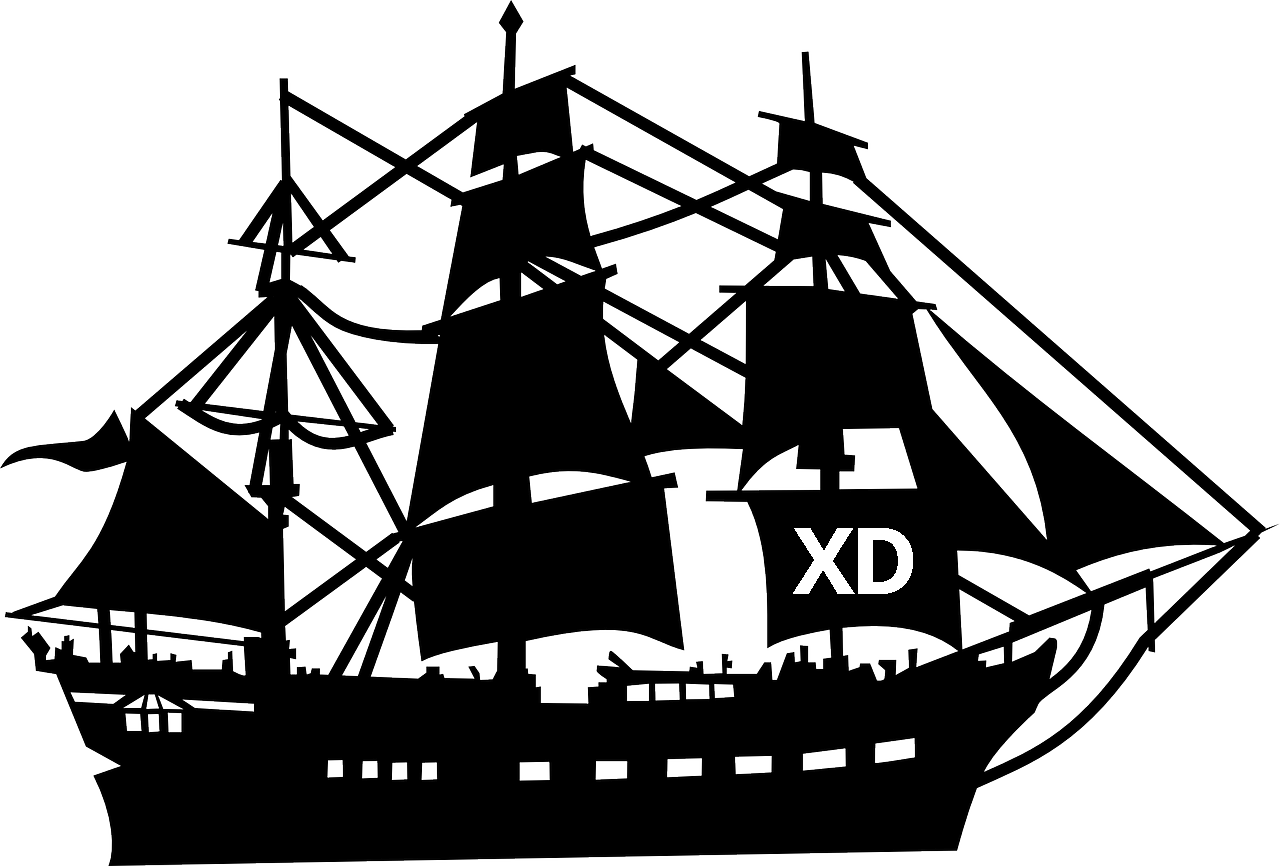
\includegraphics[height=8cm]{front-obrazek.png}

        \vspace{1.5cm}

        \Huge\textbf{Jakieś piosenki}
        
        \vspace{0.5cm}
        
        \LARGE Wydanie pierwsze
        
        \vfill

        \Large
        Wydawnictwo Kis Inkris \\
        Warszawa, 2021

        \vspace{0.5cm}

        \footnotesize
        https://github.com/dzierzanowski/spiewnik-szant
    \end{center}
\end{titlepage}

\tableofcontents

\newpage
\begin{song}{title={Kapitan Kidd}, music={North Cape}}
\begin{multicols}{2}
    \begin{chorus}
        Me ^{e}imię ^{h}William ^{e}Kidd \\
        Już czeka ^{a}stryk, czeka ^{D}stryk \\
        Królewski ^{e}korsarz ^{h}William ^{e}Kidd, czeka ^*{G}stry ^{D}k \\
        Me ^{G}imię ^{D}William ^{a}Kidd \\
        Zbrodni ^*{e}ogrom ^{h}nych to ^{a}mit \\
        Powró^{e}ciłem, ^{G}choć w Lon^{h}dynie ^{D/F#}czeka ^{e}stryk
    \end{chorus}
    \begin{verse}
        Mój ^{e}ojciec ^{h}uczył ^{e}mnie \\
        Jak nie ^{G}znaleźć się na ^{D}dnie \\
        Lecz los o^{e}krutny ^{D}zabrał ^{a}go ro^{h}dzinie ^{e}mej \\
        Choć biblię w ^{e}rękę ^{h}moją ^{e}kładł \\
        Morza ^{G}urok na mnie ^{D}padł \\
        I mary^{e}narzem ^{D}stałem ^{a}się, choć ^{h}czeka ^{e}stryk
    \end{verse}
    \begin{chorus}
        Me imię William Kidd\ldots
    \end{chorus}
    \begin{verse}
        Kanonier William Moore \\
        Pierwszy trafił na mój sznur \\
        Bo przeciw mnie ośmielił się on wzniecić bunt \\
        Choć dobrym strzelcem William był \\
        Pod salingiem będzie gnił \\
        Buntownik każdy skończy tak, już czeka stryk
    \end{verse}
    \begin{chorus}
        Me imię William Kidd\ldots
    \end{chorus}
    \begin{verse}
        Raz gdy było ze mną źle \\
        Obiecałem sobie, że \\
        Mądrości drogą odtąd pójdę po kres dni \\
        Lecz mój korsarski podły fach \\
        Zabił wnet o duszę strach \\
        I potępienie czeka mnie, bo czeka stryk
    \end{verse}
    \begin{chorus}
        Me imię William Kidd\ldots
    \end{chorus}
    \begin{verse}
        \textit{(wolniej)} \\
        To egzekucyjny blok \\
        Zaraz mnie ogarnie mrok \\
        Bo na mą szyję kat założy gruby sznur \\
        Więc dzisiaj ostrzec ciebie chcę \\
        Byś za przykład nie brał mnie \\
        Mądrości drogą zawsze szedł, bo czeka stryk
    \end{verse}
    \begin{chorus}
        \textit{(szybciej)} \\
        Me imię William Kidd\ldots
    \end{chorus}
\end{multicols}
\end{song}
\newpage

\newpage
\begin{song}{title={Stary bryg}, music={EKT Gdynia}}
    \begin{intro}
        \writechord{d} \writechord{a} \writechord{d} \writechord{G} $\times 2$
    \end{intro}
    \begin{verse}
        ^{d} Gdy wy^{a}pływał z ^{d}portu ^{a}stary bryg ^{d} ^{a} ^{d} ^{G} \\
        ^{d}Jego ^{C}dalszych ^{F}losów ^{C}nie znał ^{d}nikt ^{a} ^{d} ^{G} \\
        ^{d}Nikt nie wiedział ^{F}o tym, że \\
        ^{G}Statkiem-widmem ^{a}stanie się stary ^{d}bryg ^{a} ^{d} ^{G} \\
        ^{d} ^{a} ^{d} ^{G}
    \end{verse}
    \begin{chorus}
        ^{d}Hej, ^{F}ho! ^{C}na umrzyka ^{d}skrzyni \\
        ^{F}I bu^{C}telka ^{d}rumu ^{a} ^{d} ^{G} \\
        ^{d}Hej, ^{F}ho! ^{C}resztę czas u^{d}czyni \\
        ^{F}I bu^{C}telka ^{d}rumu ^{a} ^{d} ^{G} \\
        ^{d} ^{a} ^{d} ^{G}
    \end{chorus}
    \begin{verse}
        Co z załogą zrobił stary bryg \\
        Tego też nie zgadnie chyba nikt \\
        Czy zostawił w porcie ją \\
        Czy na morza dnie? Nikt nie wie gdzie
    \end{verse}
    \begin{chorus}
        Hej, ho! na umrzyka skrzyni\ldots
    \end{chorus}
    \begin{verse}
        Przepowiednia zła jest, że ho ho \\
        Kto go spotka, marny jego los \\
        Ale my nie martwmy się \\
        Hej, nie martwmy się --- rum jeszcze jest!
    \end{verse}
    \begin{chorus}
        Hej, ho! na umrzyka skrzyni\ldots $\times 2$ 
    \end{chorus}
\end{song}



\newpage
\pagestyle{empty}
\mbox{}
\cleardoublepage{}

\end{document}
